%% -*- coding: utf-8 -*-
\documentclass[12pt,a4paper]{scrartcl} 
\usepackage[utf8]{inputenc}
\usepackage[english,russian]{babel}
\usepackage{indentfirst}
\usepackage{misccorr}
\usepackage{graphicx}
\usepackage{amsmath}
\begin{document}
	\begin{titlepage}
		\begin{center}
			\large
			МИНИСТЕРСТВО НАУКИ И ВЫСШЕГО ОБРАЗОВАНИЯ РОССИЙСКОЙ ФЕДЕРАЦИИ
			
			Федеральное государственное бюджетное образовательное учреждение высшего образования
			
			\textbf{АДЫГЕЙСКИЙ ГОСУДАРСТВЕННЫЙ УНИВЕРСИТЕТ}
			\vspace{0.25cm}
			
			Инженерно-физический факультет
			
			Кафедра управления и информатики в технических системах
			\vfill
			
			\vfill
			
			\textsc{Отчет по практике}\\[5mm]
			
			{\LARGE Программаная реализация численного метода \textit{Вычисление матрицы обратной заданной.}}
			\bigskip
			
			1 курс, группа 1УТС
		\end{center}
		\vfill
		
		\newlength{\ML}
		\settowidth{\ML}{«\underline{\hspace{0.7cm}}» \underline{\hspace{2cm}}}
		\hfill\begin{minipage}{0.5\textwidth}
			Выполнил:\\
			\underline{\hspace{\ML}} В.\,М.~Карпенко\\
			«\underline{\hspace{0.7cm}}» \underline{\hspace{2cm}} 2022 г.
		\end{minipage}%
		\bigskip
		
		\hfill\begin{minipage}{0.5\textwidth}
			Руководитель:\\
			\underline{\hspace{\ML}} С.\,В.~Теплоухов\\
			«\underline{\hspace{0.7cm}}» \underline{\hspace{2cm}} 2022 г.
		\end{minipage}%
		\vfill
		
		\begin{center}
			Майкоп, 2022 г.
		\end{center}
	\end{titlepage}

	\section{Введение}
	\label{sec:intro}
	
	% Что должно быть во введении
	\begin{enumerate}
		\item Текстовая формулировка задачи
		\item Пример кода, решающего данную задачу
		\item График
		\item Скриншот программы
	\end{enumerate}
	
	Пример приведен в пункте ~\ref{sec:exp} на стр.~\pageref{sec:exp}.
	
	\section{Ход работы}
	\label{sec:exp}
	
	\subsection{Код приложения}
	\label{sec:exp:code}
	\begin{verbatim}
		#include <iostream>
#include <ctime>
#include <cmath>

using namespace std;

template <typename T> void FreeMem(T** matr, int n);
template <typename T> void PrintMtx(T** matr, int n);
template <typename T> void SetMtx(T** matr, int n);
template <typename T> void TransponMtx(T** matr, T** tMatr, int n);
void Get_matr(int** matr, int n, int** temp_matr, int indRow, int indCol);
int Det(int** matr, int n);

void main()
{
    srand((unsigned)time(NULL));
    setlocale(0, "");
    int n, det;
    cout << "Введите размер матрицы: ";
    cin >> n;
    int** matr = new int* [n];
    double** obr_matr = new double* [n];
    double** tobr_matr = new double* [n];
    for (int i = 0; i < n; i++) {
        matr[i] = new int[n];
        obr_matr[i] = new double[n];
        tobr_matr[i] = new double[n];
    }
    SetMtx(matr, n);
    PrintMtx(matr, n);
    det = Det(matr, n);
    cout << "Определитель матрицы = " << det << endl;
    if (det) {
        for (int i = 0; i < n; i++) {
            for (int j = 0; j < n; j++) {
                int m = n - 1;
                int** temp_matr = new int* [m];
                for (int k = 0; k < m; k++)
                    temp_matr[k] = new int[m];
                Get_matr(matr, n, temp_matr, i, j);
                obr_matr[i][j] = pow(-1.0, i + j + 2) * Det(temp_matr, m) / det;
                FreeMem(temp_matr, m);
            }
        }
    }
    else
        cout << "Т.к. определитель матрицы = 0,\nто матрица вырожденная и обратной не имеет!!!" << endl;
    //Транспонирование матрицы
    TransponMtx(obr_matr, tobr_matr, n);
    //Печать обратной матрицы после транспонирования
    PrintMtx(tobr_matr, n);
    FreeMem(tobr_matr, n);
    FreeMem(matr, n);
    FreeMem(obr_matr, n);
}
//Функция транспонирования матрицы
template <typename T> void TransponMtx(T** matr, T** tMatr, int n) {//
    for (int i = 0; i < n; i++)
        for (int j = 0; j < n; j++)
            tMatr[j][i] = matr[i][j];
}
//Функция освобождения памяти
template <typename T> void FreeMem(T** matr, int n)
{
    for (int i = 0; i < n; i++)
        delete[] matr[i];
    delete[] matr;
}

//функция заполнения матрицы
template <typename T> void SetMtx(T** matr, int n)
{
    for (int i = 0; i < n; i++)
        for (int j = 0; j < n; j++) {
            //  matr[i][j] = rand() % 9 + 1;
            cout << "Введите элемент [" << i << "," << j << "] \n";
            cin >> matr[i][j];
        }
}

//функция печати матрицы
template <typename T> void PrintMtx(T** matr, int n)
{
    for (int i = 0; i < n; i++) {
        for (int j = 0; j < n; j++)
            cout << matr[i][j] << " ";
        cout << endl;
    }
}
//функция вычеркивания строки и столбца
void Get_matr(int** matr, int n, int** temp_matr, int indRow, int indCol)
{
    int ki = 0;
    for (int i = 0; i < n; i++) {
        if (i != indRow) {
            for (int j = 0, kj = 0; j < n; j++) {
                if (j != indCol) {
                    temp_matr[ki][kj] = matr[i][j];
                    kj++;
                }
            }
            ki++;
        }
    }
}

//===========================================================
//                              вычисление определителя
//===========================================================
//функция вычисления определителя матрицы
int Det(int** matr, int n)
{
    int temp = 0;   //временная переменная для хранения определителя
    int k = 1;      //степень
    if (n < 1) {
        cout << "Не верный размер матрицы!!!" << endl;
        return 0;
    }
    else if (n == 1)
        temp = matr[0][0];
    else if (n == 2)
        temp = matr[0][0] * matr[1][1] - matr[1][0] * matr[0][1];
    else {
        for (int i = 0; i < n; i++) {
            int m = n - 1;
            int** temp_matr = new int* [m];
            for (int j = 0; j < m; j++)
                temp_matr[j] = new int[m];
            Get_matr(matr, n, temp_matr, 0, i);
            temp = temp + k * matr[0][i] * Det(temp_matr, m);
            k = -k;
            FreeMem(temp_matr, m);
        }
    }
    return temp;
}
	    
	\end{verbatim}
	
	\subsection{Пример формулы}
	\label{sec:mathexample}
	
	Нахождение обратной матрицыЖ
	\begin{equation}\label{eq:solv}
		A^{-1}=\frac{1}{|A|}*A^{S}
	    \hspace{0.5cm}
	    |A|\neq 0
	    \hspace{0.2cm}
	 \end{equation}
	Можно сослаться на уравнение~\eqref{eq:solv}.
	
\section{Пример вставки изображения}
\label{sec:picexample}
\begin{figure}[h]
	\centering
	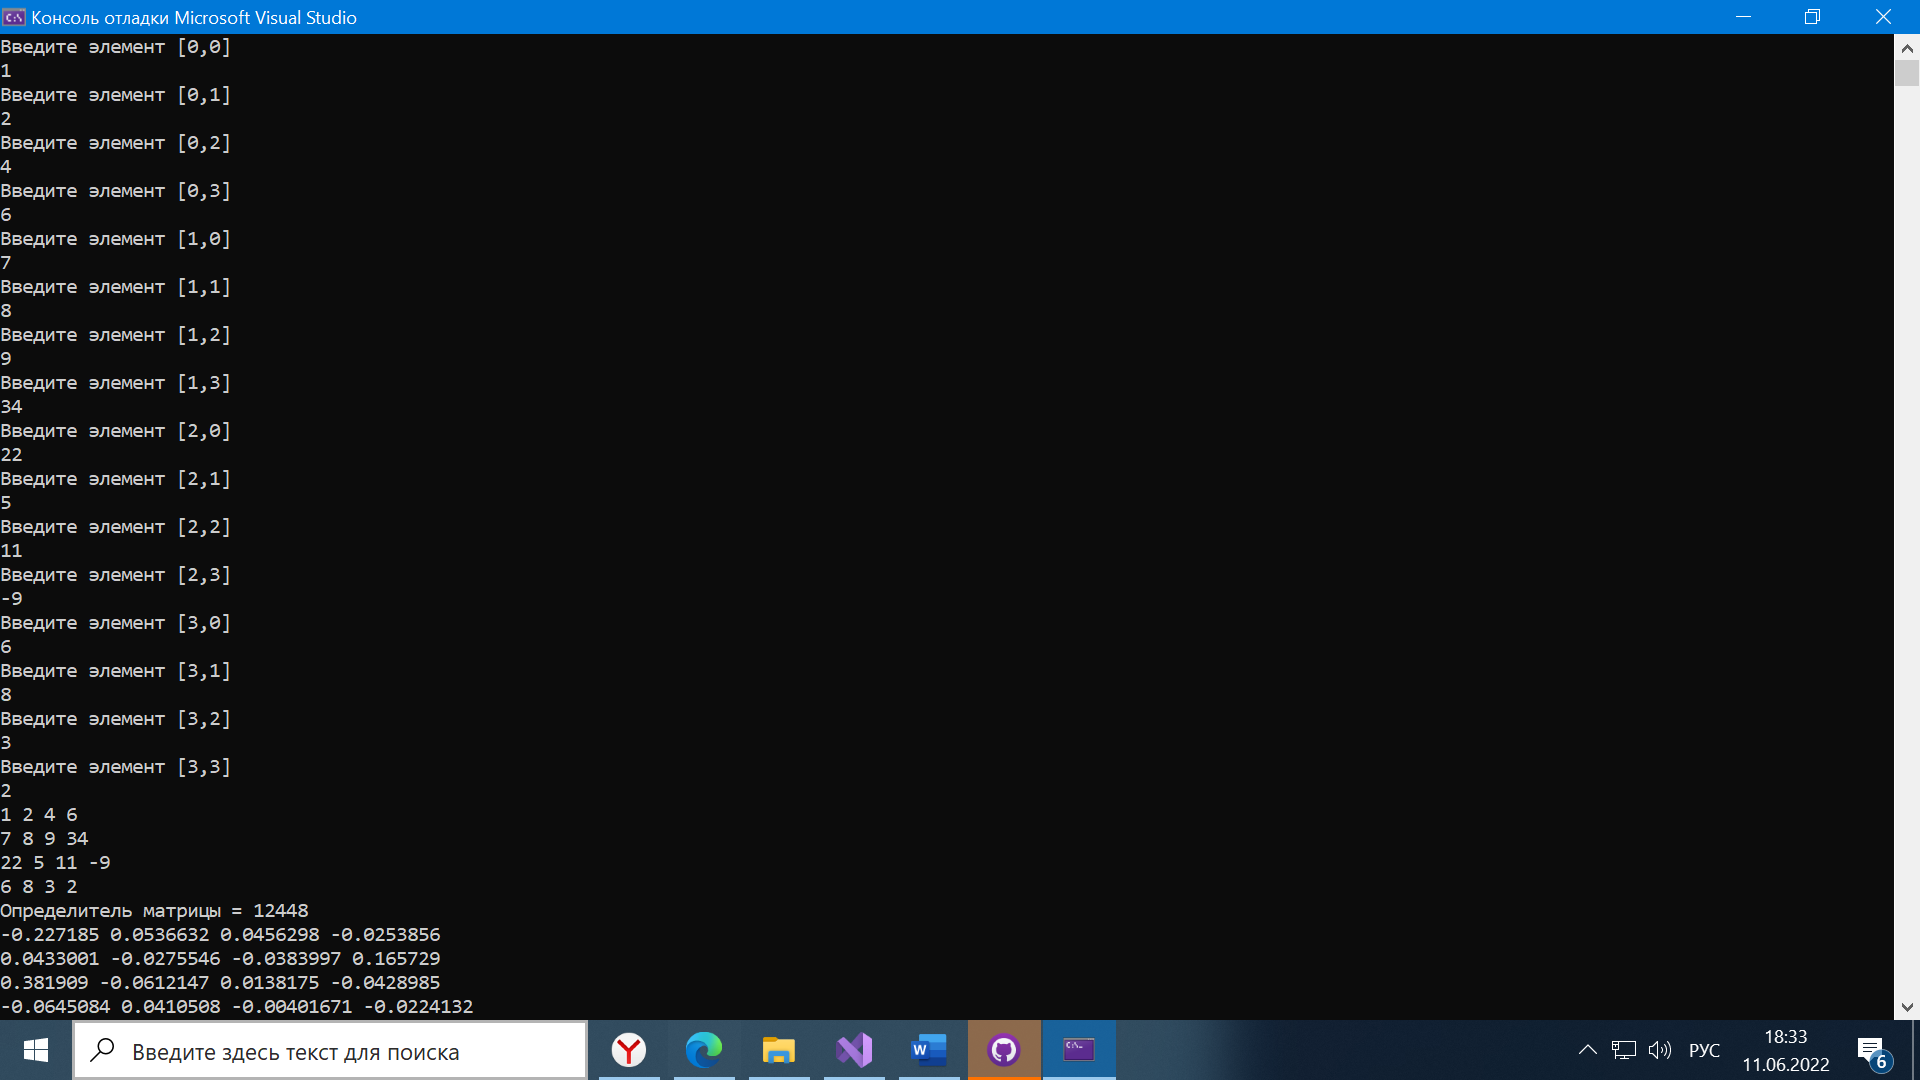
\includegraphics[width=0.4\textwidth]{screen_prog.jpg}
	\caption{Парабола}\label{fig:par}
\end{figure}
\newpage
\section{Пример библиографических ссылок}
    http://geo.phys.spbu.ru/LDUS/files/books/LaTeX/LaTeX-Lvovsky.pdf
	
	\begin{thebibliography}{9}
		\bibitem{Knuth-2003}Кнут Д.Э. Всё про \TeX. \newblock --- Москва: Изд. Вильямс, 2003 г. 550~с.
		\bibitem{Lvovsky-2003}Львовский С.М. Набор и верстка в системе \LaTeX{}. \newblock --- 3-е издание, исправленное и дополненное, 2003 г.
		\bibitem{Voroncov-2005}Воронцов К.В. \LaTeX{} в примерах. 2005 г.
	\end{thebibliography}
\end{document}